\documentclass[10pt]{IEEEtran}
\usepackage{tikz}
\usepackage{dblfloatfix}
\usepackage{amsmath}
\usepackage{subfig}
\usetikzlibrary{shapes,snakes}
\usetikzlibrary{calc,chains,positioning}
% \usetikzlibrary{external}
% \tikzexternalize[prefix=figures/]
\usepackage{phaistos}
\usepackage{graphics,color}\usepackage{cite}
\newtheorem{simulation}{Simulation}
\usepackage{url}\usepackage{pgfplots}
\usepackage[bottom]{footmisc}
\DeclareMathOperator{\diag}{diag}

\begin{document}
% \newlength\figureheight
% \newlength\figurewidth
% \setlength\figureheight{5.5cm}
% \setlength\figurewidth{6.9cm}
\urlstyle{sf}
%
\title{Regularization for Partial Multichannel Equalization for Speech Dereverberation}

\author{
  Ina~Kodrasi,~\IEEEmembership{Student~Member,~IEEE}, Stefan~Goetze,~\IEEEmembership{Member,~IEEE}, Simon~Doclo,~\IEEEmembership{Member,~IEEE}
  \thanks{Copyright (c) 2013 IEEE. Personal use of this material is permitted. However, permission to use this material for any other purposes must be obtained from the IEEE by sending a request to \underline{pubs-permission@ieee.org}.}
  \thanks{I. Kodrasi is with the Department of Medical Physics and Acoustics, Signal Processing Group, University of Oldenburg, 26111 Oldenburg, Germany (ina.kodrasi@uni-oldenurg.de).}
  \thanks{S. Goetze is with the Fraunhofer Institute Digital Media Technology, 26129 Oldenburg, Germany (s.goetze@idmt.fraunhofer.de).}
  \thanks{S. Doclo is with the Department of Medical Physics and Acoustics, Signal Processing Group, University of Oldenburg, 26111 Oldenburg, Germany and with the Fraunhofer Institute Digital Media Technology, 26129 Oldenburg, Germany (simon.doclo@uni-oldenburg.de).}%
  \thanks{This work was supported in part by a Grant from the GIF, the German-Israeli Foundation for Scientific
Research and Development and the Cluster of Excellence 1077 "Hearing4All", funded by the German Research Foundation (DFG)."}
}


% make the title area
\maketitle
\newpage

\begin{abstract}
\boldmath
Acoustic multichannel equalization techniques such as the multiple-input/output inverse theorem~(MINT), which aim to equalize the room impulse responses~(RIRs) between the source and the microphone array, are known to be highly sensitive to RIR estimation errors.
To increase robustness, it has been proposed to incorporate regularization in order to decrease the energy of the equalization filters.
In addition, more robust partial multichannel equalization techniques such as relaxed multichannel least-squares~(RMCLS) and channel shortening~(CS) have recently been proposed.

In this paper, we propose a partial multichannel equalization technique based on MINT~(P-MINT) which aims to shorten the RIR.
Furthermore, we investigate the effectiveness of incorporating regularization to further increase the robustness of P-MINT and the aforementioned partial multichannel equalization techniques, i.e. RMCLS and CS.
In addition, we introduce an automatic non-intrusive procedure for determining the regularization parameter based on the L-curve.

Simulation results using measured RIRs show that incorporating regularization in P-MINT yields a significant performance improvement in the presence of RIR estimation errors, whereas a smaller performance improvement is observed when incorporating regularization in RMCLS and CS.
Furthermore, it is shown that the intrusively regularized P-MINT technique outperforms all other investigated intrusively regularized multichannel equalization techniques in terms of perceptual speech quality~(PESQ).
Finally, it is shown that the automatic non-intrusive regularization parameter in regularized P-MINT leads to a very similar performance as the intrusively determined optimal regularization parameter, making regularized P-MINT a robust, perceptually advantageous, and practically applicable multichannel equalization technique for speech dereverberation.
\end{abstract}

\begin{IEEEkeywords}
acoustic multichannel equalization, speech dereverberation, automatic regularization
\end{IEEEkeywords}

\section{Introduction}
\IEEEPARstart{S}{PEECH} signals recorded in an enclosed space by microphones placed at a distance from the source are often corrupted by reverberation, which arises from the superposition of delayed and attenuated copies of the anechoic speech signal.
Reverberation causes signal degradation, typically leading to decreased speech intelligibility~\cite{Houtgast_1985,Beutelmann_2006} and performance deterioration in speech recognition systems~\cite{Omologo_1998, Sehr_phd, Maas_ICASSP_2012}.
Hence, many speech communication applications such as teleconferencing applications, voice-controlled systems, or hearing aids, require effective dereverberation algorithms~\cite{Sehr_phd,Jeub_ITASP_2010,Maas_ICASSP_2012}.

In the last decades, several dereverberation approaches have been developed, which can be broadly classified into speech enhancement and acoustic channel equalization approaches~\cite{Naylor_Derev_book}.
While both single and multichannel dereverberation techniques have been investigated, multichannel techniques are generally preferred since they enable the use of both spectro-temporal and spatial processing of the received microphone signals.
Well-known multichannel speech enhancement techniques for dereverberation are either based on spectral subtraction~\cite{Habets_ITASLP_2008,Habets_ICASSP_2007} or on linear prediction~\cite{Gaubitch_JASA_2006,Delcroix_2007,Nakatani_ITASLP_2010}.
Furthermore, acoustic multichannel equalization techniques~\cite{Miyoshi_ITASS_1988,Kallinger_ICASSP_2006, Hikichi_EURASIP_2007, Mertins_ITASLP_2010, Zhang_IWAENC_2010, Haque_ITASLP_2011, Kodrasi_ICASSP_2012} aim to reshape the estimated room impulse responses~(RIRs) between the source and the microphone array.
Such techniques comprise an attractive approach to speech dereverberation since in theory perfect channel equalization can be achieved~\cite{Miyoshi_ITASS_1988, Hacihabibouglu_ITASLP_2012}.

A widely known multichannel equalization technique that aims at complete equalization is the multiple-input/output inverse theorem (MINT)~\cite{Miyoshi_ITASS_1988}, which however suffers from several drawbacks in practice.
Since the estimated RIRs typically differ from the true RIRs due to fluctuations~(e.g., temperature or position variations~\cite{Radlovic_ITSA_2000}) or estimation errors~(e.g., due to the sensitivity of blind system identification~(BSI) methods to near-common zeros~\cite{Lin_ITASLP_2012} or interfering noise~\cite{Hasan_EUSIPCO_2006}), MINT fails to equalize the true RIRs, possibly leading to severe distortions in the output signal.
In an attempt to increase the robustness of MINT, it has been proposed to incorporate regularization in order to decrease the energy of the equalization filters~\cite{Hikichi_EURASIP_2007}.

In addition, more robust partial multichannel equalization techniques such as relaxed multichannel least-squares~(RMCLS)~\cite{Zhang_IWAENC_2010} and channel shortening~(CS)~\cite{Kallinger_ICASSP_2006} have recently been proposed.
Since early reflections tend to improve speech intelligibility~\cite{Arweiler_JASA_2011,Warzybok_JASA_2012} and late reverberation~(typically defined as the part of the RIR after $50$--$80$~ms) is the major cause of speech intelligibility degradation, the objective of such techniques is to shorten the RIR by suppressing only the reverberant tail.
It has been experimentally validated that partial equalization techniques lead to a significant increase in robustness in the presence of RIR estimation errors as compared to complete equalization~\cite{Zhang_IWAENC_2010}.
However, by not imposing any constraints on the remaining early reflections of the shortened RIR, RMCLS and CS may lead to undesired perceptual effects.

In this paper, we first introduce a partial multichannel equalization technique based on MINT~(P-MINT), which aims to shorten the RIR and to directly control the perceptual speech quality~\cite{Kodrasi_ICASSP_2012}.
Furthermore, since incorporating regularization is also expected to further increase the robustness of partial multichannel equalization techniques, the effectiveness of incorporating regularization in all aforementioned techniques is investigated.
To this end, a regularization term proportional to the energy of the reshaping filters is added to the cost functions for P-MINT, RMCLS, and CS.
Whereas a closed-form solution exists for minimizing the regularized cost functions for P-MINT and RMCLS, an iterative approach is required for minimizing the regularized cost function for CS.

In general, the optimal regularization parameter yielding the highest perceptual speech quality needs to be determined intrusively~(i.e. using a dereverberated reference signal and knowledge of the true RIRs), limiting the practical applicability of the regularized techniques.
In this paper, we also propose and extensively investigate an automatic non-intrusive selection procedure for the regularization parameter based on the L-curve~\cite{Hansen_1993}.

Using simulations with a realistic acoustic system in the presence of estimation errors, it is shown that a significant performance increase is obtained for P-MINT when regularization is incorporated, whereas a smaller improvement is observed for RMCLS and CS.
In addition, it is demonstrated that the intrusively regularized P-MINT technique outperforms the intrusively regularized RMCLS and CS techniques, typically leading to the highest robustness and perceptual speech quality.
Furthermore, it is shown that the non-intrusively determined regularization parameter yields a nearly optimal perceptual speech quality in regularized P-MINT, making it a robust, perceptually advantageous, and practically applicable multichannel equalization technique for speech dereverberation.

The paper is organized as follows.
In Section~\ref{sec: intro} the acoustic multichannel equalization problem is introduced as well as several state-of-the-art multichannel equalization  techniques for designing reshaping filters.
A mathematical relation between the P-MINT solution and the multiple possible CS solutions is provided, showing that the P-MINT solution can be expressed as a linear combination of the CS solutions.
Furthermore, the incorporation of a regularization term in all multichannel equalization techniques is discussed in Section~\ref{sec: reg}, whereas in  Section~\ref{sec: sel_reg} an automatic non-intrusive procedure for computing the regularization parameter is proposed.
Using simulations, the reverberant tail suppression and the perceptual speech quality of all considered equalization techniques is extensively compared in Section~\ref{sec: exp}.

\section{Acoustic Multichannel Equalization}
\label{sec: intro}
In this section, complete and partial acoustic multichannel equalization techniques are discussed.
First, the general problem is stated and some notational conventions are given.
Then the cost functions of several multichannel equalization techniques are discussed.

\subsection{Problem Formulation and Notation}
\label{subsec: prob}
Consider an acoustic system with a single speech source and $M$ microphones as depicted in Fig.~\ref{fig: acsys}.
The $m$-th microphone signal, $m = 1, \; \ldots, \; M$, at time index $n$ is given by
\begin{figure}[b]
  \centering
  %\tikzsetnextfilename{configuration}
  %\input{Plots/configuration.tikz}
  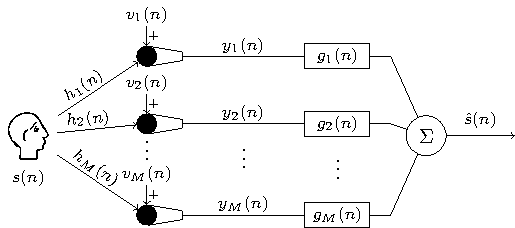
\includegraphics[scale=0.9]{figures/configuration.pdf}
  \caption{Multichannel equalization system}
  \label{fig: acsys}
\end{figure}
\begin{equation}
  y_m(n) =  \underbrace{s(n) \ast h_m(n)}_{x_m(n)} + v_m(n) = x_m(n) + v_m(n),
\end{equation}
where $\ast$ denotes convolution, $s(n)$ is the clean speech signal, $h_m(n)$ denotes the RIR between the source and the $m$-th microphone, and $v_m(n)$ is the additive noise signal.
Since acoustic multichannel equalization techniques generally design reshaping filters disregarding the presence of noise, in the following it is assumed that $v_m(n) = 0$, hence $y_m(n) = x_m(n)$.

The RIR can be described in vector notation as $\mathbf{h}_m = \left[h_m(0) \; h_m(1) \; \ldots \; h_m(L_h-1) \right]^T$, with $L_h$ being the RIR length and $\left[\cdot \right]^T$ denoting the transpose operation.
Given reshaping filters $\mathbf{g}_m$ of length $L_g$, i.e. $\mathbf{g}_m = \left[g_m(0) \; g_m(1) \; \ldots \; g_m(L_g-1) \right]^T$, the output signal $\hat{s}(n)$ of the multichannel equalization system is given by the sum of the filtered microphone signals, i.e.
\begin{equation}
  \hat{s}(n) = \sum_{m=1}^{M} x_m(n) \ast g_m(n) = s(n) \ast \underbrace{\sum_{m=1}^{M} h_m(n) \ast g_m(n)}_{c(n)},
\end{equation}
where $c(n)$ is the equalized impulse response~(EIR) between the source and the output of the system.
The EIR can be described in vector notation as $\mathbf{c} = \left[c(0) \; c(1) \; \ldots \; c(L_c-1) \right]^{T}$, with $L_c = L_h+L_g-1$ being the EIR length.
Using the $ML_g$--dimensional stacked filter vector $\mathbf{g}$, i.e.
\begin{equation}
  \mathbf{g}  =  \left[\mathbf{g}_1^T \; \mathbf{g}_2^T \; \ldots \; \mathbf{g}_M^T \right]^T,
\end{equation}
 and the $L_c \times ML_g$--dimensional multichannel convolution matrix $\mathbf{H}$, i.e.
\begin{equation}
\mathbf{H}  = \left[\mathbf{H}_1 \; \mathbf{H}_2 \; \ldots \; \mathbf{H}_M \right],
\end{equation}
with
\begin{equation}
\small
\mathbf{H}_m =  \begin{bmatrix}
    h_m(0) & 0 &  \ldots & 0 \\
    h_m(1) & h_m(0) & \ddots & \vdots \\
    \vdots & h_m(1) & \ddots & 0 \\
    h_m(L_h-1) & \vdots & \ddots & h_m(0) \\
    0 & h_m(L_h-1) & \ddots & h_m(1) \\
    \vdots & \ddots & \ddots & \vdots \\
    0 & \ldots & 0 & h_m(L_h-1)
   \end{bmatrix},\hspace{-0.4cm}
 \end{equation}
the output signal can be expressed as
\begin{align}
\hat{s}(n) &=  \sum_{m=1}^{M} \mathbf{g}_m^T
 \mathbf{H}_m^T
\underbrace{\left[
\begin{array}{c}
s(n) \\
s(n-1) \\
\vdots \\
s(n-L_c+1) \\
\end{array}
\right]}_{\mathbf{s}(n)}  \\
& =  \mathbf{g}^T \mathbf{H}^T \mathbf{s}(n)  =  \mathbf{c}^T \mathbf{s}(n).
\end{align}
The reshaping filter $\mathbf{g}$ can then be constructed based on different design objectives for the EIR
\begin{equation}
\boxed{\mathbf{c} = \mathbf{H}\mathbf{g}}
\end{equation}
Since the true RIRs are typically not available in practice, acoustic multichannel equalization techniques design the reshaping filter $\mathbf{g}$ using the estimated multichannel convolution matrix $\hat{\mathbf{H}}$ constructed from the estimated RIRs
\begin{equation}
\label{eq: hath}
\hat{h}_m(n) = h_m(n) + e_m(n),
\end{equation}
with $e_m(n)$ representing the estimation error.
The sensitivity of several multichannel equalization techniques to these estimation errors will be investigated in Section~\ref{sec: exp}.


\subsection{Complete Multichannel Equalization}
\label{subsec: mint}
The objective of complete multichannel equalization techniques such as MINT is to invert the acoustic system up to a delay, such that the output of the system is a shifted version of the clean speech signal.
\subsubsection*{Multiple-input/output inverse theorem~\cite{Miyoshi_ITASS_1988}}
MINT aims to recover the delayed anechoic speech signal by designing a filter $\mathbf{g}$ such that
\begin{equation}
  \label{eq: minttar}
  \hat{\mathbf{H}}\mathbf{g} = \mathbf{d},
\end{equation}
where $\mathbf{d}$ is the desired EIR defined as a delayed impulse, i.e.
\begin{equation}
  \mathbf{d} = [\underbrace{0 \; \ldots \; 0}_{\tau} \; 1 \; 0 \; \ldots \; 0 ],
\end{equation}
with $\tau$ being the delay in number of samples.
The inverse filter is then computed by minimizing the least-squares cost function
\begin{equation}
\label{eq: ls}
\boxed{J_{_{\rm MINT}}(\mathbf{g}) = \|\hat{\mathbf{H}}\mathbf{g} - \mathbf{d}\|_2^2}
\end{equation}
As shown in~\cite{Miyoshi_ITASS_1988}, assuming that
\begin{itemize}
  \item the estimated RIRs do not share any common zeros in the $z$-plane, and
  \item $L_g \geq \lceil{\frac{L_h-1}{M-1}\rceil}$,
\end{itemize}
where $\lceil{ \cdot \rceil}$ denotes the ceiling function, the filter that inverts the multichannel acoustic system can be computed as
\begin{equation}
  \label{eq: mint}
  \boxed{\mathbf{g}_{{}_{\rm MINT}} = \hat{\mathbf{H}}^+\mathbf{d}}
\end{equation}
with $\{\cdot\}^+$ denoting the Moore-Penrose pseudo-inverse.
Since the estimated convolution matrix $\hat{\mathbf{H}}$ is assumed to be a full row-rank matrix~\cite{Harikumar_ITSP_1998}, its pseudo-inverse can be computed as $\hat{\mathbf{H}}^+ = \hat{\mathbf{H}}^T(\hat{\mathbf{H}}\hat{\mathbf{H}}^T)^{-1}$.

When the RIRs are perfectly estimated, MINT achieves perfect equalization.
However, when the estimated RIRs differ from the true RIRs, the resulting EIR $\mathbf{c} = \mathbf{H} \hat{\mathbf{H}}^+ \mathbf{d}$ not only differs from the desired response $\mathbf{d}$, but usually causes large distortions in the output signal~\cite{Radlovic_ITSA_2000, Hikichi_EURASIP_2007}.


\subsection{Partial Multichannel Equalization}
\label{sec: partial}
Whereas MINT is very sensitive to estimation errors, partial multichannel equalization techniques which aim at reshaping the EIR instead of complete equalization, are significantly more robust.
The recently proposed partial multichannel equalization techniques such as RMCLS and CS aim at suppressing the late reverberation only, while imposing no constraints on the early reflections, which may lead to undesired perceptual effects.
Therefore we also introduce a partial multichannel equalization technique based on MINT, which aims at simultaneously suppressing the reverberant tail as well as directly controlling the perceptual speech quality of the output signal.

\subsubsection*{Relaxed multichannel least-squares~\cite{Zhang_IWAENC_2010}}
RMCLS achieves partial equalization by introducing a weighting vector $\mathbf{w}$ in the least-squares cost function in~(\ref{eq: ls}), i.e. the RMCLS cost function is defined as
\begin{equation}
\label{eq: rmcls_cost}
\boxed{J_{_{\rm RMCLS}}(\mathbf{g}) = \|\mathbf{W}(\hat{\mathbf{H}}\mathbf{g} - \mathbf{d})\|_2^2}
\end{equation}
with $\mathbf{W} = {\diag}\{\mathbf{w}\}$, and the weighting vector $\mathbf{w}$ equal to
\begin{equation}
\mathbf{w} = [\underbrace{1 \; \ldots \; 1}_{\tau} \; \underbrace{1 \; 0 \; \ldots \; 0}_{L_s} \; 1 \; \ldots 1]^{T},
\end{equation}
where $L_s$ denotes the length of the direct path and early reflections in number of samples.
The minimization of~(\ref{eq: rmcls_cost}) aims at setting the reverberant tail of the EIR to $\mathbf{0}$, while the first taps corresponding to the early reflections are not constrained.
Similarly to the MINT solution in~(\ref{eq: mint}), the reshaping filter minimizing the RMCLS cost function in~(\ref{eq: rmcls_cost}) can be computed as
\begin{equation}
\boxed{\mathbf{g}_{{}_{\rm RMCLS}} = (\mathbf{W}\hat{\mathbf{H}})^{+}\mathbf{W}\mathbf{d}}
\end{equation}

\subsubsection*{Channel shortening~\cite{Kallinger_ICASSP_2006}}
CS has been extensively investigated in the context of digital communication applications~\cite{Martin_ITSP_2005} and has recently been applied to acoustic system equalization in~\cite{Kallinger_ICASSP_2006, Zhang_IWAENC_2010}.
CS is achieved by maximizing the energy in the first $L_s$ taps of the EIR (i.e. direct path and early reflections), while minimizing the energy in the remaining taps (i.e. reverberant tail).
This optimization problem is expressed as the maximization of a generalized Rayleigh quotient, i.e.
\begin{equation}
\label{eq: rayleigh}
\boxed{J_{_{\rm CS}} (\mathbf{g}) =  \frac{\|{\diag}\{\mathbf{w}_d\}\hat{\mathbf{H}}\mathbf{g}\|_2^2}{\|{\diag}\{\mathbf{w}_u\}\hat{\mathbf{H}}\mathbf{g}\|_2^2} = \frac{\mathbf{g}^T \hat{\mathbf{B}} \mathbf{g}}{\mathbf{g}^T \hat{\mathbf{A}} \mathbf{g}}}
\end{equation}
where $\mathbf{w}_d$ and $\mathbf{w}_u$ represent the desired and undesired window respectively, i.e.
\begin{align}
\label{eq: wincs}
\mathbf{w}_d & = [\underbrace{0 \; \ldots \; 0}_{\tau} \; \underbrace{1 \; \ldots \; 1}_{L_s}\; 0\; \ldots\; 0]^{T}  \\
\mathbf{w}_u & = [\underbrace{1 \; \ldots \; 1}_{\tau} \; \underbrace{0 \; \ldots \; 0}_{L_s}\; 1\; \ldots\; 1]^{T} = \mathbf{1} - \mathbf{w}_d,
\end{align}
and
\begin{align}
\hat{\mathbf{B}} & = \hat{\mathbf{H}}^{T} {\diag}\{\mathbf{w}_d \}^T{\diag}\{\mathbf{w}_d \}\hat{\mathbf{H}}  \\
\hat{\mathbf{A}} & = \hat{\mathbf{H}}^{T} {\diag}\{\mathbf{w}_u \}^T{\diag}\{\mathbf{w}_u \}\hat{\mathbf{H}}.
\end{align}
Maximizing~(\ref{eq: rayleigh}) is equivalent to solving the generalized eigenvalue problem $\hat{\mathbf{B}} \mathbf{g} = \lambda \hat{\mathbf{A}} \mathbf{g}$, where the optimal reshaping filter $\mathbf{g}_{_{\rm CS}}$ is the generalized eigenvector corresponding to the largest generalized eigenvalue $\lambda_{\max}$, i.e.
\begin{equation}
\label{eq: cssol}
\boxed{\hat{\mathbf{B}} \mathbf{g}_{_{\rm CS}} = \lambda_{\max} \hat{\mathbf{A}}\mathbf{g}_{_{\rm CS}}}
\end{equation}
Designing the reshaping filter using such an energy-based optimization technique however imposes no other, e.g. perceptually relevant, constraints on the remaining filter taps of the EIR, which may lead to undesired perceptual effects~(cf. Section~\ref{sec: regacsys}).
Furthermore, multiple solutions to~(\ref{eq: cssol}) exist~(cf. Section~\ref{sec: pmint_and_cs}), and each of these solutions will lead to a perceptually different EIR.
In~\cite{Zhang_IWAENC_2010} it has been proposed to select the generalized eigenvector leading to the minimum $l_2$-norm estimated EIR.
In this paper, the intrusively selected generalized eigenvector leading to the highest perceptual speech quality has been used~(cf. Section~\ref{sec: acsys}).
\subsubsection*{Partial multichannel equalization based on MINT~\cite{Kodrasi_ICASSP_2012}}
In order to directly control the perceptual quality of the output signal, we recently proposed the P-MINT technique, where the direct path and early reflections of the EIR are controlled by using the first part of one of the estimated RIRs as the desired EIR in~(\ref{eq: minttar}), i.e.
\begin{equation}
\label{eq: PMINT}
\hat{\mathbf{H}} \mathbf{g} = \hat{\mathbf{h}}_{p}^{\rm d},
\end{equation}
where
\begin{equation}
\label{eq: tarpmint}
\hat{\mathbf{h}}_{p}^{\rm d} = [\underbrace{0\phantom{\rlap{$(L_s-1)$}} \ldots 0 }_{\tau} \underbrace{\hat{h}_p(0) \ldots \hat{h}_p(L_s-1)}_{L_s} 0 \ldots 0 ]^{T},
\end{equation}
with $p \in \{1, \; 2, \; \ldots, \; M \}$.
Without loss of generality, also other desired EIRs could be used instead of~(\ref{eq: tarpmint}), as long as they are perceptually close to the true RIRs.
The least-squares cost function to be minimized in P-MINT is hence defined as
\begin{equation}
\label{eq: pmintcost}
\boxed{J_{_{\rm P-MINT}}(\mathbf{g}) = \|\hat{\mathbf{H}}\mathbf{g} - \hat{\mathbf{h}}_p^{\rm d}\|_2^2}
\end{equation}
Assuming that the same conditions as for MINT are satisfied, the reshaping filter minimizing~(\ref{eq: pmintcost}) can be computed as
\begin{equation}
\label{eq: Pmintsol}
\boxed{\mathbf{g}_{{}_{\rm P-MINT}} = \hat{\mathbf{H}}^{+}\hat{\mathbf{h}}_p^{\rm d}}
\end{equation}

\subsection{Relation Between P-MINT and CS}
\label{sec: pmint_and_cs}
Following similar arguments as in~\cite{Zhang_IWAENC_2010}, a mathematical relation between the P-MINT solution and the multiple possible CS solutions can be derived.

The maximization of the CS cost function in~(\ref{eq: rayleigh}) can be reformulated as computing a filter $\mathbf{g}$ belonging to the null space of $\hat{\mathbf{A}}$ but not belonging to the null space of $\hat{\mathbf{B}} + \hat{\mathbf{A}}$, i.e. satisfying the system of equations
\begin{equation}
\label{eq: sys}
\begin{cases}
\mathbf{g}^T (\hat{\mathbf{B}} + \hat{\mathbf{A}})\mathbf{g} \neq 0 \\
\mathbf{g}^T\hat{\mathbf{A}} \mathbf{g} = 0,
\end{cases}
\end{equation}
 with $\hat{\mathbf{B}} + \hat{\mathbf{A}} = \hat{\mathbf{H}}^T\hat{\mathbf{H}}$.
Since the convolution matrix $\hat{\mathbf{H}}$ is assumed to be a full row-rank matrix with ${\rm rank}(\hat{\mathbf{H}}) = L_c$, also ${\rm rank}(\hat{\mathbf{B}} + \hat{\mathbf{A}}) = L_c$.
Exploiting the relationship between the rank and the dimension of the null space of a matrix~\cite{Golub_Matrix_book}, the dimension of the null space of $\hat{\mathbf{B}} + \hat{\mathbf{A}}$ is equal to
\begin{eqnarray}
{\rm dim}[{\rm Nullspace} (\hat{\mathbf{B}} + \hat{\mathbf{A}})] = ML_g - L_c,
\end{eqnarray}
where $\rm{dim}[ \cdot]$ denotes the dimension of the considered space.
In addition, since ${\rm rank}(\hat{\mathbf{A}}) = {\rm rank}(\hat{\mathbf{H}}^T \hat{\mathbf{H}}) - L_s = L_c - L_s$, the dimension of the null space of $\hat{\mathbf{A}}$ is equal to
\begin{eqnarray}
{\rm dim}[{\rm Nullspace} (\hat{\mathbf{A}})] = ML_g - (L_c - L_s).
\end{eqnarray}
Hence, the number of linearly independent vectors satisfying~(\ref{eq: sys}) and therefore maximizing the generalized Rayleigh quotient in~(\ref{eq: rayleigh}) is $[ML_g-(L_c-L_s)] - [ML_g-L_c] = L_s$.

In order to derive a mathematical relation between the P-MINT solution and the multiple possible CS solutions, consider that the desired EIR in P-MINT can be expressed as
\begin{equation}
\hat{\mathbf{h}}_p^{\rm d} = {\diag}\{\mathbf{w}_d \}\hat{\mathbf{h}}_p,
\end{equation}
with $\mathbf{w}_d$ defined in~(\ref{eq: wincs}).
For the filter $\mathbf{g}_{{}_{\rm P-MINT}}$ in~(\ref{eq: Pmintsol}), the denominator of the Rayleigh quotient in~(\ref{eq: rayleigh}) is equal to
\begin{align}
\mathbf{g}_{{}_{\rm P-MINT}}^T \hat{\mathbf{A}} \mathbf{g}_{{}_{\rm P-MINT}} &= \|{\diag}\{\mathbf{w}_{u}\}\hat{\mathbf{H}} \hat{\mathbf{H}}^+\hat{\mathbf{h}}_p^d \|_2^2 \\
& =  \|{\diag}\{\mathbf{w}_{u}\} {\diag} \{\mathbf{w}_d \} \hat{\mathbf{h}}_p\|_2^2 = 0,
\end{align}
whereas the nominator in~(\ref{eq: rayleigh}) is equal to
\begin{align}
\mathbf{g}_{{}_{\rm P-MINT}}^T \hat{\mathbf{B}} \mathbf{g}_{{}_{\rm P-MINT}} & = \|{\diag}\{\mathbf{w}_{d}\}\hat{\mathbf{H}} \hat{\mathbf{H}}^+\hat{\mathbf{h}}_p^{\rm d} \|_2^2 \\
& =  \|{\diag}\{\mathbf{w}_{d}\} \hat{\mathbf{h}}_p^{\rm d} \|_2^2 \neq 0.
\end{align}
Therefore since the P-MINT filter satisfies~(\ref{eq: sys}), it is also in the solution space of the CS optimization problem.
As a result, the P-MINT reshaping filter can be expressed as a linear combination of the $L_s$ generalized eigenvectors maximizing the generalized Rayleigh quotient in~(\ref{eq: rayleigh}).

\section{Regularization in Acoustic Multichannel Equalization}
\label{sec: reg}
As previously mentioned, the estimated RIRs $\hat{h}_m(n)$ generally differ from the true RIRs~(cf.~(\ref{eq: hath})).
Since the reshaping filters $\mathbf{g}_m$ are designed using the estimated RIRs, the output signal of the multichannel equalization system is given by
\begin{align}
\hat{s}(n) \!  & = \! s(n) \! \ast \! \! \sum_{m=1}^M \!\! h_m(n) \ast g_m(n) + \sum_{m=1}^M \!\! v_m(n) \ast g_m(n) \\
& = \! s(n) \! \ast \! \! \sum_{m=1}^M \!\!\!\left[\hat{h}_m(n) - e_m(n)\right] \!\!\ast\! g_m(n)\! + \! \sum_{m=1}^M \! \! v_m(n) \ast g_m(n)\!\!  \\ 
\label{eq: 2}
& = s(n) \! \ast \! \sum_{m=1}^M \! \! \hat{h}_m(n) \ast g_m(n) \\
\label{eq: 3}
& - s(n) \! \ast \! \sum_{m=1}^M \!\! e_m(n) \ast g_m(n) \! + \! \sum_{m=1}^M \!\! v_m(n) \ast g_m(n),
\end{align}
where the term in~(\ref{eq: 2}) represents the clean speech signal convolved with the desired EIR and the remaining terms in~(\ref{eq: 3}) may~(and typically do) give rise to large signal distortions due to RIR estimation errors and the additive noise.
However, if the energy of the filters $g_m(n)$ is small, then the value of these distortion terms is also small.
To increase the robustness of MINT, it has therefore been proposed to add a regularization term
\begin{equation}
\label{eq: regterm}
J_{\rm reg} = \delta \|\mathbf{g}\|_2^2
\end{equation}
to the cost function in~(\ref{eq: ls}), with the aim of decreasing the energy of the filter $\mathbf{g}$.
The regularization parameter $\delta$ controls the weight given to the minimization of the energy of the inverse filter.
In this paper, we will investigate the effectiveness of incorporating the regularization term $J_{\rm reg}$ in all partial multichannel equalization techniques discussed in Section~\ref{sec: intro}.
Moreover, in Section~\ref{sec: sel_reg} the computation of the regularization parameter $\delta$ is discussed, where both an optimal intrusive computation procedure as well as an automatic non-intrusive procedure is proposed.
As previously mentioned, acoustic multichannel equalization techniques generally design reshaping filters disregarding the presence of noise, hence in the following it is again assumed that $v_m(n) = 0$.
\subsubsection*{Regularized MINT~\cite{Hikichi_EURASIP_2007}}
In the regularized MINT technique, the least-squares cost function in~(\ref{eq: ls}) is extended to
\begin{equation}
\label{eq: cost_rmint}
\boxed{J_{{}_{\rm MINT}}^{^{_{\rm R}}}(\mathbf{g}) = \|\hat{\mathbf{H}}\mathbf{g} - \mathbf{d}\|_2^2 + \delta \|\mathbf{g} \|_2^2}
\end{equation}
such that the regularized MINT filter minimizing this cost function is equal to
\begin{equation}
\label{eq: rmint_sgol}
\boxed{\mathbf{g}_{{}_{\rm MINT}}^{{_{\rm R}}}  = (\hat{\mathbf{H}}^T\hat{\mathbf{H}}+\delta \mathbf{I})^{-1}\hat{\mathbf{H}}^{T}\mathbf{d}}
\end{equation}
with $\mathbf{I}$ being the $ML_g\times ML_g$-dimensional identity matrix.
In~\cite{Hikichi_EURASIP_2007} it has been shown that incorporating regularization in MINT is useful in reducing the distortions in the output signal due to fluctuations of the RIRs.


\subsubsection*{Regularized RMCLS}
Since RMCLS is a least-squares technique, incorporating the regularization term $J_{\rm reg}$ can be done similarly as for MINT.
The regularized RMCLS cost function to be minimized is defined as
\begin{equation}
\label{eq: cost_rrmcls}
\boxed{J_{{}_{\rm RMCLS}}^{^{_{\rm R}}}(\mathbf{g}) =  \|\mathbf{W}({\hat{\mathbf{H}}}\mathbf{g} - \mathbf{d})\|_2^2 + \delta \|\mathbf{g} \|_2^2}
\end{equation}
and the regularized RMCLS filter minimizing this cost function can be calculated as
\begin{equation}
\boxed{\mathbf{g}_{{}_{\rm RMCLS}}^{{_{\rm R}}}  = [(\mathbf{W}\hat{\mathbf{H}})^T(\mathbf{W}\hat{\mathbf{H}}) + \delta \mathbf{I}]^{-1} (\mathbf{W}\hat{\mathbf{H}})^T \mathbf{W}\mathbf{d}}
\end{equation}

\subsubsection*{Regularized P-MINT}
Similarly to the regularized least-squares technique for MINT and RMCLS, the regularized P-MINT cost function is defined as
\begin{equation}
\label{eq: cost_rpmint}
\boxed{J_{{}_{\rm P-MINT}} ^{^{_{\rm R}}}(\mathbf{g}) = \|\hat{\mathbf{H}}\mathbf{g} - \hat{\mathbf{h}}_p^{\rm d}\|_2^2 + \delta \|\mathbf{g} \|_2^2}
\end{equation}
Minimizing~(\ref{eq: cost_rpmint}) yields the regularized P-MINT filter
\begin{equation}
\label{eq: rpmintsol}
\boxed{\mathbf{g}_{{}_{\rm P-MINT}}^{{_{\rm R}}}  = (\hat{\mathbf{H}}^T\hat{\mathbf{H}}+\delta \mathbf{I})^{-1}\hat{\mathbf{H}}^{T}\hat{\mathbf{h}}_p^{\rm d}}
\end{equation}

\subsubsection*{Regularized CS}
In order to incorporate the regularization term $J_{\rm reg}$ in CS, the maximization problem in~(\ref{eq: rayleigh}) is first reformulated in terms of a generalized Rayleigh quotient \emph{minimization} problem, such that the regularized CS cost function to be minimized can be defined as
\begin{equation}
\label{eq: cost_rcs}
\boxed{J_{{}_{\rm CS}}^{^{_{\rm R}}}(\mathbf{g})= \frac{\mathbf{g}^T {\hat{\mathbf{A}}} \mathbf{g}}{\mathbf{g}^T {\hat{\mathbf{B}}} \mathbf{g}} + \delta \|\mathbf{g} \|_2^2}
\end{equation}
However, since no analytical solution to minimize~(\ref{eq: cost_rcs}) exists, an iterative optimization technique for minimizing this non-linear cost function will be used in the following.
In order to improve the numerical robustness and the convergence speed of the optimization technique, the gradient
\begin{equation}
\frac{\partial J_{{}_{\rm CS}}^{^{_{\rm R}}}(\mathbf{g})}{\partial \mathbf{g}} = 2 \left[ \frac{(\mathbf{g}^T \hat{\mathbf{B}} \mathbf{g})\hat{\mathbf{A}}\mathbf{g} - (\mathbf{g}^T \hat{\mathbf{A}} \mathbf{g})\hat{\mathbf{B}}\mathbf{g} }{(\mathbf{g}^T \hat{\mathbf{B}} \mathbf{g})^2} +  \delta \mathbf{g} \right],
\end{equation}
and the Hessian
\begin{equation}
\begin{split}
& \frac{\partial ^2 J_{{}_{\rm CS}}^{^{_{\rm R}}}(\mathbf{g})}{\partial^2 \mathbf{g}}  = \\
& 2 \left[ \frac{(\mathbf{g}^T \hat{\mathbf{B}} \mathbf{g}) \hat{\mathbf{A}} - (\mathbf{g}^T \hat{\mathbf{A}} \mathbf{g}) \hat{\mathbf{B}} + 2 ( \hat{\mathbf{A}} \mathbf{g} \mathbf{g}^T \hat{\mathbf{B}} - \hat{\mathbf{B}} \mathbf{g} \mathbf{g}^T \hat{\mathbf{A}})}{(\mathbf{g}^T \hat{\mathbf{B}}\mathbf{g})^2} \right. \\
& \left. -  4 \frac{[(\mathbf{g}^T\hat{\mathbf{B}}\mathbf{g})\hat{\mathbf{A}}\mathbf{g} - (\mathbf{g}^T\hat{\mathbf{A}}\mathbf{g})\hat{\mathbf{B}}\mathbf{g}] \mathbf{g}^T \hat{\mathbf{B}}}{(\mathbf{g}^T\hat{\mathbf{B}}\mathbf{g})^3} + \delta \mathbf{I} \right],
\end{split}
\end{equation}
can be provided.

Since the non-linear cost function in~(\ref{eq: cost_rcs}) typically contains local minima, it should be noted that this technique is sensitive to the initial vector provided to the numerical optimization algorithm.
In an attempt to find the global minimum, we have considered different initial vectors, i.e. one of the generalized eigenvector $\mathbf{g}_{_{\rm CS}}$ solving~(\ref{eq: cssol}), the P-MINT solution $\mathbf{g}_{{}_{\rm P-MINT}}$ in~(\ref{eq: Pmintsol}), and the vector $[1 \; 0 \; \ldots \; 0]^T$.
The optimal solution is then selected as the one leading to the highest perceptual speech quality~(cf. Section~\ref{sec: acsys}).


\section{Non-intrusive Selection of the Regularization Parameter}
\label{sec: sel_reg}
Increasing the regularization parameter $\delta$ in all regularized equalization techniques presented in Section~\ref{sec: reg} decreases the norm of the reshaping filter $\mathbf{g}$, increasing the robustness to RIR estimation errors.
However, increasing this parameter also reduces the equalization performance with respect to the true RIRs, resulting in a trade-off between equalization performance for perfectly estimated RIRs and robustness in the presence of RIR estimation errors.

Obviously, different values of the regularization parameter $\delta$ lead to different performance.
The optimal value $\delta_{\rm opt}$ that yields the highest perceptual speech quality depends on the acoustic system to be equalized, the RIR estimation errors, as well as the equalization technique being used.
While in simulations $\delta_{\rm opt}$ can be intrusively determined exploiting the known true RIRs~(cf. Section~\ref{sec: regacsys}), an automatic non-intrusive procedure is required in practice.

For conciseness, the automatic non-intrusive procedure for selecting the regularization parameter in acoustic multichannel equalization techniques is discussed only for the regularized P-MINT technique.
However, the procedure proposed here can be extended to any regularized least-squares technique, such as regularized MINT and regularized RMCLS.\footnote{The presented approach cannot be used for the regularized CS technique. Automatic selection of the regularization parameter in CS remains a topic for future investigation.}

Incorporating regularization in P-MINT introduces a trade-off between minimizing the residual energy $\|\hat{\mathbf{H}}\mathbf{g} - \hat{\mathbf{h}}_p^{\rm d} \|_2^2$ and minimizing the filter energy $\|\mathbf{g}\|_2^2$~(cf.~(\ref{eq: cost_rpmint})).
A good regularization parameter should hence incorporate knowledge about both the residual energy and the filter energy, such that both energies are kept small.
In order to automatically compute a regularization parameter for regularized least-squares problems, it has been proposed in~\cite{Hansen_1993} to use a parametric plot of the solution norm versus the residual norm for several values of $\delta$.
This plot always has an L-shape with the corner~(i.e. the point of maximum curvature) located exactly where the regularized least-squares solution changes in nature from being dominated by over-regularization to being dominated by under-regularization.

We therefore propose selecting the regularization parameter $\delta_{\rm auto}$ in the regularized P-MINT technique as the one corresponding to the corner of the parametric plot of the filter norm $\|\mathbf{g}_{{}_{\rm P-MINT}}^{_{\rm R}}\|_2$ versus the residual norm $\|\hat{\mathbf{H}}\mathbf{g}_{{}_{\rm P-MINT}}^{_{\rm R}} - \hat{\mathbf{h}}_p^{\rm d}\|_2$.
As is experimentally validated in Section~\ref{sec: exp}, such a regularization parameter also leads to a nearly optimal perceptual speech quality.

The L-curve can be generated by computing the reshaping filter $\mathbf{g}_{{}_{\rm P-MINT}}^{_{\rm R}}$ in~(\ref{eq: rpmintsol}) for several values of the regularization parameter $\delta$ and then calculating the required norms.
However, in order to reduce the computational complexity, it is beneficial to generate the L-curve using the singular value decomposition~(SVD) of the estimated convolution matrix $\hat{\mathbf{H}}$.
Consider the SVD of $\hat{\mathbf{H}}$, i.e.
\begin{equation}\label{eq: svd}
  \hat{\mathbf{H}} = \hat{\mathbf{U}}\hat{\mathbf{S}}\hat{\mathbf{V}}^T,
\end{equation}
where $\hat{\mathbf{U}}$ and $\hat{\mathbf{V}}$ are orthogonal matrices and $\hat{\mathbf{S}}$ is a diagonal matrix containing the singular values $\hat{\sigma}_k$ of $\hat{\mathbf{H}}$ in descending order, i.e. $\hat{\mathbf{S}} = {\diag}\{\left[\hat{\sigma}_1 \; \hat{\sigma}_2 \; \ldots \; \hat{\sigma}_{L_c}\right]\}$.
Using~(\ref{eq: rpmintsol}) and~(\ref{eq: svd}), the regularized P-MINT filter can be expressed as
\begin{equation}
\mathbf{g}_{{}_{\rm P-MINT}}^{_{\rm R}}  =  \sum_{k=1}^{L_c} \frac{\hat{\sigma}_k \hat{\mathbf{u}}_k^T \hat{\mathbf{h}}_p^{\rm d} }{\hat{\sigma}_k^2+\delta}  \hat{\mathbf{v}}_k,
\end{equation}
where $\hat{\mathbf{u}}_k$ and $\hat{\mathbf{v}}_k$ denote the $k$-th column of $\hat{\mathbf{U}}$ and $\hat{\mathbf{V}}$ respectively.
Hence, for a given $\delta$, the filter norm and the residual norm can be expressed in terms of the singular values/vectors as
\begin{equation}
\label{eq: eta}
\boxed{\|\mathbf{g}_{{}_{\rm P-MINT}}^{_{\rm R}}\|_2 = \sqrt{\sum_{k = 1}^{L_c} \frac{\hat{\sigma}_k^2 (\hat{\mathbf{u}}_k^T \hat{\mathbf{h}}_p^{\rm d})^2}{(\hat{\sigma}_k^2 + \delta)^2}}}
\end{equation}
\begin{equation}
\label{eq: rho}
\boxed{ \|\hat{\mathbf{H}}\mathbf{g}_{{}_{\rm P-MINT}}^{_{\rm R}} - \hat{\mathbf{h}}_p^{\rm d}\|_2 = \sqrt{\sum_{k = 1}^{L_c} \frac{\delta^2 (\hat{\mathbf{u}}_k^T \hat{\mathbf{h}}_p^{\rm d})^2}{(\hat{\sigma}_k^2 + \delta)^2}}}
\end{equation}
Therefore, once the SVD is computed, the complete L-curve can be readily generated using~(\ref{eq: eta}) and~(\ref{eq: rho}).

\begin{figure}[t!]
  \centering
  %\tikzsetnextfilename{lcurve_ex}
  %% This file was created by matlab2tikz v0.4.0.
% Copyright (c) 2008--2013, Nico Schlömer <nico.schloemer@gmail.com>
% All rights reserved.
% 
% The latest updates can be retrieved from
%   http://www.mathworks.com/matlabcentral/fileexchange/22022-matlab2tikz
% where you can also make suggestions and rate matlab2tikz.
% 
% 
% 
\begin{tikzpicture}[font = \small]

\begin{axis}[%
width=\figurewidth,
height=\figureheight,
scale only axis,
xmin=-0.005,
xmax=0.12,
xtick = {0, 0.02, 0.04, 0.06, 0.08, 0.1, 0.12},
xticklabels = {0, 0.02, 0.04, 0.06, 0.08, 0.1},
xlabel={Least-squares error},
xmajorgrids,
ymin=-5000,
ymax=120000,
ytick = {0,20000,40000,60000,80000,100000},
ylabel={Condition number},
ylabel absolute, ylabel style={yshift=-1.0em},
xlabel style={yshift=0.2em, align = center},
ymajorgrids
]
\addplot [
color=blue,
dashed,
line width=1.2pt,
mark size=2.2pt,
mark=o,
mark options={solid},
forget plot
]
table[row sep=crcr]{
0.101683347794715 619.327594930765\\
0.070745345298329 910.163142451782\\
0.0518215776650418 1446.05932037595\\
0.034064480268289 2236.23282740251\\
0.021490164999668 3212.3656467179\\
0.0146601306623177 4065.52058480655\\
0.00974151392832193 5104.23809281723\\
0.0063666801741859 7587.91061319979\\
0.00413442371755222 10938.5138981644\\
0.0028143172811875 15047.1511902914\\
0.00179731470310589 20720.8208654107\\
0.00107409629745723 42007.5584351387\\
0.000651664771825611 102481.015352579\\
};
\addplot [
color=green!50!black,
only marks,
mark=square*,
mark size=1.5pt,
thick,
mark options={solid},
]
table[row sep=crcr]{
0.00413442371755222 10938.5138981644\\
};
\addplot [
color=red,
only marks,
mark=asterisk,
mark size=2.3pt,
thick,
mark options={solid},
]
table[row sep=crcr]{
0.000651664771825611 102481.015352579\\
};
\addplot [
color=yellow!30!black,
only marks,
mark=triangle*,
mark size=2.3pt,
thick,
mark options={solid},
]
table[row sep=crcr]{
0.101683347794715 619.327594930765\\
};
\node at (axis cs:0.003, 105000) [anchor=west] {\color{red}{$L^{\rm t}_w = 1947$}}; 
\node at (axis cs:0.09, 17000) [anchor=west] {\color{yellow!30!black}{$L^{\rm s}_w = 300$}}; 
\node at (axis cs:0.008, 20000) [anchor=west] {\color{green!50!black}{$L^{\rm s}_w = 1000$}}; 
\end{axis}
\end{tikzpicture}%
  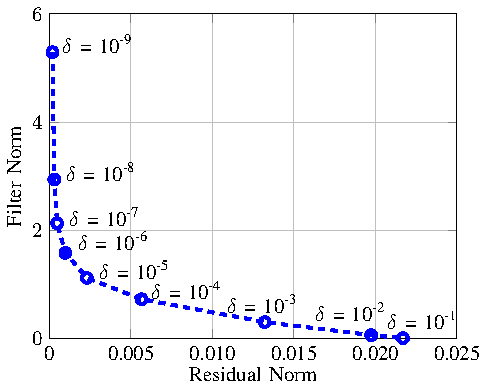
\includegraphics[scale=0.9]{figures/lcurve_ex.pdf}
  \caption{Typical L-curve obtained using regularized P-MINT for an erroneously estimated acoustic system}
  \label{fig: lcurveex}
\end{figure}
Fig.~\ref{fig: lcurveex} depicts a typical L-curve obtained using regularized P-MINT for equalizing an estimated acoustic system~(cf. Section~\ref{sec: acsys}).
As illustrated in this figure, increasing the value of $\delta$ decreases the filter norm but at the same time increases the residual norm.
Although from such a curve it seems easy to determine the regularization parameter that corresponds to the maximum curvature, numerical problems due to small singular values may occur and hence, a numerically stable algorithm is required.
In this work, the triangle method~\cite{Castellanos_2002} is used for locating the point of maximum curvature of the L-curve.

\section{Simulations}
\label{sec: exp}

In this section, simulation results for a scenario with a single speech source and $2$ microphones are presented.
In Section~\ref{sec: acsys}, the acoustic systems and the used performance measures are introduced.
In Section~\ref{sec: regacsys}, the performance of all equalization techniques and their regularized counterparts with the intrusively determined regularization parameter $\delta_{\rm opt}$ is compared in the presence of channel estimation errors.
% It will be shown that the regularized P-MINT technique yields the highest perceptual speech quality among all considered multichannel equalization techniques for different RIR estimation errors and values of the desired window length $L_s$.
In Section~\ref{sec: auto}, the performance of regularized P-MINT when using the automatic non-intrusive procedure for determining the regularization parameter $\delta_{\rm auto}$ instead of using $\delta_{\rm opt}$ is extensively investigated.
%It will be shown that using the regularization parameter $\delta_{\rm auto}$ yields a nearly optimal performance in the regularized P-MINT technique.
Finally, in Section~\ref{sec: noise}, the performance of P-MINT and automatically regularized P-MINT in the presence of both channel estimation errors and additive noise will be investigated.
Sound samples from each simulation can be found at {\small \url{www.sigproc.uni-oldenburg.de/audio/dereverb/pmint.html}}.

\subsection{Acoustic System and Performance Measures}
\label{sec: acsys}
We have considered an acoustic scenario with a single speech source and $M=2$ omni-directional microphones placed at a distance of $2.3$~m from the source in a room with reverberation time $T_{\rm 60} \approx 550$~ms~(in Section~\ref{sec: auto}, also rooms with reverberation times $T_{60} \approx 450$~ms and $T_{60} \approx 750$~ms have been considered).
The RIRs between the source and the microphones have been measured using the swept-sine technique~\cite{Farina_2000} and the RIR length has been set to $L_h = 4400$ at a sampling frequency $f_s = 16$~kHz.
In order to simulate estimation errors, the measured RIRs have been perturbed by adding scaled white noise as proposed in~\cite{Cho_ITSA_1999}, i.e.
\begin{equation}
  \label{eq: he}
  \hat{h}_m(n) = h_m(n) + \underbrace{e(n)h_m(n)}_{e_m(n)}
\end{equation}
with $e(n)$ being an uncorrelated Gaussian noise sequence with zero mean and an appropriate variance, such that a desired \emph{normalized channel mismatch} $E_m$, defined as
\begin{equation}
  \label{eq: em}
E_m = 10 \log_{10} \frac{\|\mathbf{h}_m - \hat{\mathbf{h}}_m \|_2^2}{\|\mathbf{h}_m\|_2^2},
\end{equation}
is generated.
\begin{figure*}[b!]
  \centering
  \hbox{\subfloat[\label{fig: edcnoreg33a}]{%
      %\tikzsetnextfilename{EDC_noreg_sys_3_Cm_-33_Ld_800}
      %\input{Plots/EDC_noreg_sys_3_Cm_-33_Ld_800.tikz}
      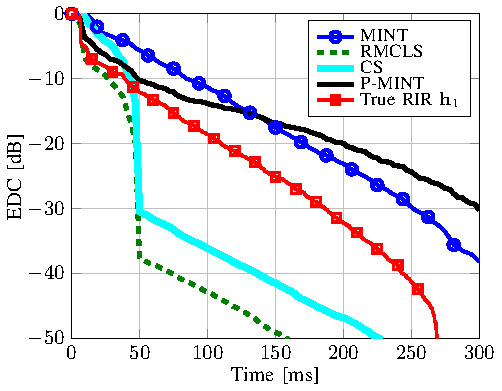
\includegraphics[scale=0.9]{figures/EDC_noreg_sys_3_Cm_-33_Ld_800.pdf}
    }
    \hspace{2cm}
    \subfloat[\label{fig: edcnoreg33b}]{%
      %\tikzsetnextfilename{EDC_reg_sys_3_Cm_-33_Ld_800}
      %\input{Plots/EDC_reg_sys_3_Cm_-33_Ld_800.tikz}
      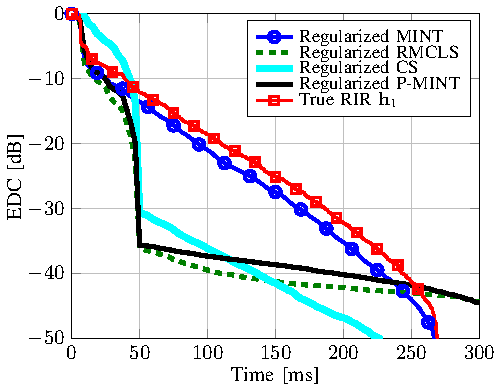
\includegraphics[scale=0.9]{figures/EDC_reg_sys_3_Cm_-33_Ld_800.pdf}
    }}
  \caption{EDC of the true RIR $\mathbf{h}_1$ and EDC of the EIR obtained using MINT, RMCLS, CS, and P-MINT (a) without regularization and (b) with optimal regularization~($E_m = -33$~dB, $L_d = 50$~ms)}
\end{figure*}
In practice, BSI methods~\cite{Hasan_EUSIPCO_2006,Haque_ITASLP_2011} should be used to directly estimate the acoustic system. 
However, to the best of our knowledge the performance of state-of-the-art BSI methods highly depends on the considered acoustic system and no model has been established to systematically describe the estimation errors that such methods yield.
Therefore,~(\ref{eq: he}) and~(\ref{eq: em}) are used to generate the considered estimation errors in the following simulations.

The simulation parameters for all considered multichannel equalization techniques are set to  $L_g = 4399$ and $\tau = 0$.
Furthermore, $5$ different desired window lengths for the partial equalization techniques are investigated, i.e. $L_d \in \{ 10~{\rm ms}, 20~{\rm ms}, 30~{\rm ms}, 40~{\rm ms}, 50~{\rm ms} \}$, with $L_d = \frac{L_s \times 10^3}{f_s}$ being the desired window length in ms.
The desired EIR in P-MINT and regularized P-MINT is chosen as the direct path and early reflections of the estimated first RIR, i.e.~$\hat{\mathbf{h}}_1^{\rm d}$.

The performance of all considered equalization techniques is evaluated both in terms of reverberant tail suppression and perceptual speech quality.
The reverberant tail suppression is evaluated using the \emph{energy decay curve}~(EDC)~\cite{Naylor_Derev_book} of the EIR defined as
\begin{equation}
{\rm EDC}(n) = 10 \log_{10} \frac{1}{\|\mathbf{c}\|_2^2} \sum_{i = n}^{L_c-1} c^2(i), \; n =0, \; \ldots, \; L_c-1,
\end{equation}
where $\mathbf{c} = \mathbf{H}\mathbf{g}$ and the reshaping filter $\mathbf{g}$ is designed using the estimated RIRs $\hat{\mathbf{h}}_m$.

The perceptual speech quality of the output signal $\hat{s}(n)$ is evaluated using the objective speech quality measure PESQ~\cite{PESQ}, which generates a similarity score between the output signal and a reference signal in the range of $1$ to $4.5$.
It has been shown in~\cite{Goetze_AES_2010} that measures relying on auditory models such as PESQ exhibit the highest correlation with subjective listening tests when evaluating the quality of dereverberated speech.
The reference signal employed here is $s(n) \ast h_1^{\rm d}(n)$, i.e. the clean speech signal convolved with the first part of the true first RIR~(which is different for each value of the desired window length $L_d$).
It should be noted that with increasing $L_d$, the reference signal becomes more similar to the unprocessed microphone signal.

As already mentioned in Section~\ref{sec: partial}, for the CS technique multiple possible solutions exist.
Out of these solutions, we have intrusively selected the generalized eigenvector leading to the highest PESQ score.


Furthermore, in order to evaluate the effectiveness of incorporating regularization in all multichannel equalization techniques, a set of regularization parameters have been considered, i.e. $\delta \in \{0, \; 10^{-9}, \; 10^{-8}, \; \ldots, \; 10^{-1} \}$, and the optimal parameter $\delta_{\rm opt}$ is selected as the one leading to the highest perceptual speech quality, i.e. PESQ score.
It should be noted that the computation of the PESQ score for selecting the optimal regularization parameter is an intrusive procedure that is not applicable in practice, since knowledge of the true RIRs is required in order to compute the reference signal $s(n) \ast h_1^{\rm d}(n)$ and the true EIR $c(n) = h(n) \ast g(n)$.
However, with the aim of illustrating the full potential of incorporating regularization in acoustic multichannel equalization techniques, the results presented in Section~\ref{sec: regacsys} are generated using such an optimal regularization parameter, whereas in Section~\ref{sec: auto} the performance when using the automatic non-intrusive procedure for the selection of the regularization parameter will be investigated.

\subsection{Optimal Regularization in the Presence of Channel Estimation Errors}
\label{sec: regacsys}
For the sake of clarity and in order to avoid overcrowded plots, these simulations are structured into two parts, with a different normalized channel mismatch in each part.
In the first simulation, a moderate mismatch $E_m = -33$~dB is considered, whereas in the second simulation a larger mismatch $E_m = -15$~dB is considered.

\begin{figure*}[b!]
  \centering
  \hbox{\subfloat[\label{fig: pesq33a}]{%
      %\tikzsetnextfilename{PESQ_noreg_sys_3_error_-33}
      %\input{Plots/PESQ_noreg_sys_3_error_-33.tikz}
      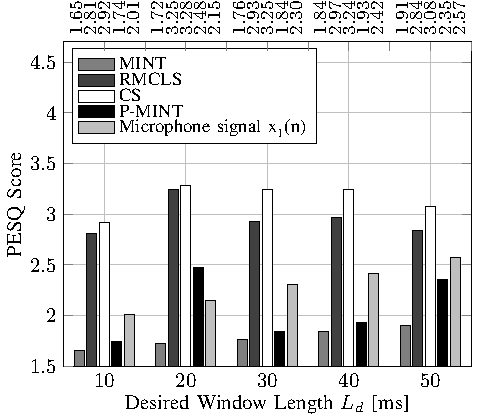
\includegraphics[scale=0.9]{figures/PESQ_noreg_sys_3_error_-33.pdf}
    }
    \hspace{2cm}
    \subfloat[\label{fig: pesq33b}]{%
      %\tikzsetnextfilename{PESQ_reg_sys_3_error_-33}
      %\input{Plots/PESQ_reg_sys_3_error_-33.tikz}
      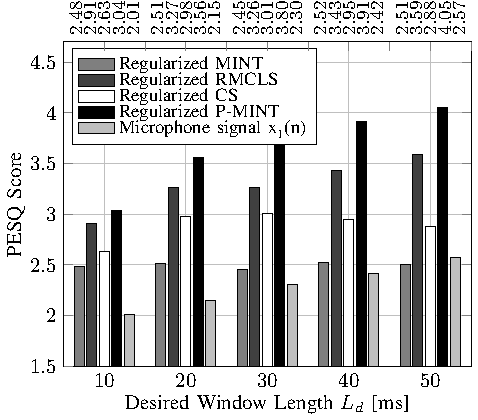
\includegraphics[scale=0.9]{figures/PESQ_reg_sys_3_error_-33.pdf}
    }}
  \caption{PESQ score of the first microphone signal $x_1(n)$ and PESQ score of the system's output $\hat{s}(n)$ obtained for several $L_d$ using MINT, RMCLS, CS, and P-MINT (a) without regularization and (b) with optimal regularization~($E_m = -33$~dB)}
\end{figure*}


\begin{simulation}[$E_m=-33$~dB]
\label{sim1} 
Fig.~\ref{fig: edcnoreg33a} depicts the EDCs of the EIRs obtained using MINT, RMCLS, CS, and P-MINT for $L_d = 50$~ms.
It can be seen that both MINT and P-MINT fail to equalize the acoustic system, leading to an EDC that is higher than the EDC of the true RIR $\mathbf{h}_1$.
On the other hand, RMCLS and CS are more robust, with their reverberant tails being below $-30$~dB.
In order to evaluate the effectiveness of incorporating regularization in all equalization techniques, Fig.~\ref{fig: edcnoreg33b} depicts the EDCs obtained using regularized MINT, regularized RMCLS, regularized CS, and regularized P-MINT with the optimal intrusively determined regularization parameter $\delta_{\rm opt}$.
As illustrated in this figure, the regularized MINT technique still fails to equalize the acoustic system.
On the contrary, all regularized partial multichannel equalization techniques are significantly more robust, providing a similar performance in terms of reverberant tail suppression.
Comparing Fig.~\ref{fig: edcnoreg33a} and Fig.~\ref{fig: edcnoreg33b}, it can be noticed that a significant improvement is obtained when incorporating regularization in P-MINT, while even a slight performance deterioration can be observed for RMCLS.
This performance deterioration can be explained by the fact that $\delta_{\rm opt}$ is selected such that the PESQ score is maximized, imposing no other constraints on the reverberant tail suppression.
Furthermore, the performance of CS does not change when regularization is incorporated, since the exhaustive comparison of the PESQ scores that each regularization parameter yields favors the intrusively selected generalized eigenvector obtained from the CS solution, hence, $\delta_{\rm opt} = 0$.

Since different EIRs leading to different perceptual speech quality may have very similar EDCs~(which is the case for all regularized partial multichannel equalization techniques in this simulation), we have also evaluated the perceptual speech quality using PESQ for different desired window lengths $L_d$ ranging from $10$~ms to $50$~ms.
The PESQ score of the first microphone signal $x_1(n)$ is also computed in order to determine the effectiveness of applying such dereverberation techniques to the system.
Fig.~\ref{fig: pesq33a} depicts the PESQ scores obtained for all considered equalization techniques without regularization, whereas Fig.~\ref{fig: pesq33b} depicts the PESQ scores when regularization is incorporated.
From Fig.~\ref{fig: pesq33b} it can be seen that the regularized P-MINT technique outperforms all other investigated regularized techniques leading to the highest PESQ score for all considered $L_d$.
Comparing the results in Fig.~\ref{fig: pesq33a} and~\ref{fig: pesq33b}, it is clear that incorporating regularization yields no performance improvement for CS, whereas the performance of MINT, RMCLS, and P-MINT is increased.
For a precise numerical comparison, the exact change in the PESQ score for all considered techniques and desired window lengths when incorporating regularization is presented in Table~\ref{tbl: pesq1}, with the maximum improvement for each desired window length indicated in bold.
\begin{table}[b!]
\centering
\caption{PESQ score improvement when incorporating regularization in MINT, RMCLS, CS, and P-MINT for several $L_d$~($E_m = -33$~dB)}
\label{tbl: pesq1}
\begin{tabular}{|l|r|r|r|r|r|r|r|r|}
\hline
$L_d$ [ms] & $10$ & $20$ & $30$ & $40$ & $50$ & Average  \\
\hline
MINT & $0.83$ & $0.79$ & $0.69$ & $0.68$ & $0.60$ & $0.72$ \\
\hline
RMCLS & $0.11$ & $0.02$ & $0.33$ & $0.47$ & $0.74$ & $0.33$ \\
\hline
CS & $0.00$ & $0.00$ & $0.00$ & $0.00$ & $0.00$ & $0.00$ \\
\hline
P-MINT & $\bf{1.30}$ & $\bf{1.08}$ & $\bf{1.95}$ & $\bf{1.98}$ & $\bf{1.70}$ & $\bf{1.60}$ \\
\hline
\end{tabular}
\end{table}
\begin{figure*}[t!]
\centering
\hbox{\subfloat[\label{fig: edcnoreg15a}]{%
    %\tikzsetnextfilename{EDC_noreg_sys_3_Cm_-15_Ld_800}
    %\input{Plots/EDC_noreg_sys_3_Cm_-15_Ld_800.tikz}
    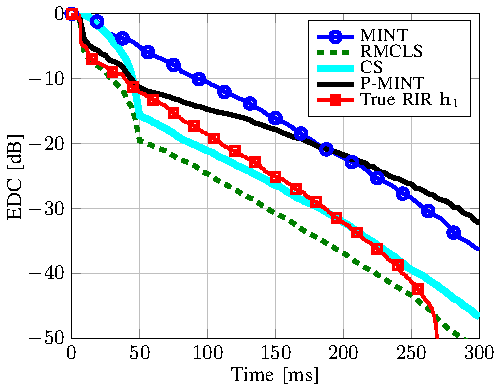
\includegraphics[scale=0.9]{figures/EDC_noreg_sys_3_Cm_-15_Ld_800.pdf}
  }
  \hspace{2cm}
  \subfloat[\label{fig: edcnoreg15b}]{%
    %\tikzsetnextfilename{EDC_reg_sys_3_Cm_-15_Ld_800}
    %\input{Plots/EDC_reg_sys_3_Cm_-15_Ld_800.tikz}
    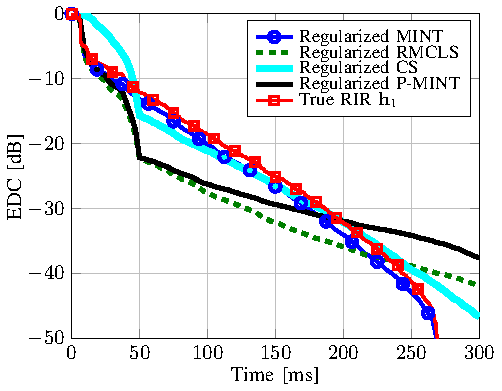
\includegraphics[scale=0.9]{figures/EDC_reg_sys_3_Cm_-15_Ld_800.pdf}
  }}
\caption{EDC of the true RIR $\mathbf{h}_1$ and EDC of the EIR obtained using MINT, RMCLS, CS, and P-MINT (a) without regularization and (b) with optimal regularization~($E_m = -15$~dB, $L_d = 50$~ms)}
\end{figure*}
Additionally, the average improvement over all considered $L_d$ values is also presented in the last column.
As previously observed, regularization is particularly useful for P-MINT, leading to an average PESQ score improvement of $1.60$.
Furthermore, also the regularized MINT and the regularized RMCLS techniques lead to a higher performance as compared to MINT and RMCLS respectively, whereas no improvement is observed in CS.
\end{simulation}
\begin{simulation}[$E_m=-15$~dB]
\label{sim2}
\begin{figure*}[t!]
  \centering
  \hbox{\subfloat[\label{fig: pesq15a}]{%
      %\tikzsetnextfilename{PESQ_noreg_sys_3_error_-15}
      %\input{Plots/PESQ_noreg_sys_3_error_-15.tikz}
      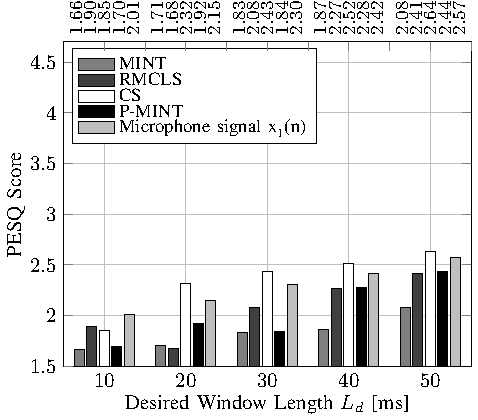
\includegraphics[scale=0.9]{figures/PESQ_noreg_sys_3_error_-15.pdf}
    }
    \hspace{2cm}
    \subfloat[\label{fig: pesq15b}]{%
      %\tikzsetnextfilename{PESQ_reg_sys_3_error_-15}
      %\input{Plots/PESQ_reg_sys_3_error_-15.tikz}
      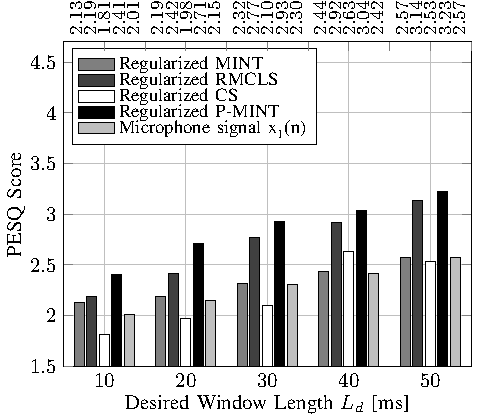
\includegraphics[scale=0.9]{figures/PESQ_reg_sys_3_error_-15.pdf}
    }}
  \caption{PESQ score of the first microphone signal $x_1(n)$ and PESQ score of the system's output $\hat{s}(n)$ obtained for several $L_d$ using MINT, RMCLS, CS, and P-MINT (a) without regularization and (b) with optimal regularization~($E_m = -15$~dB)}
\end{figure*}
In this simulation, similar analysis as in Simulation~\ref{sim1} will be conducted for the normalized channel mismatch $E_m = -15$~dB.
The EDCs obtained for $L_d = 50$~ms using MINT, RMCLS, CS, and P-MINT without regularization are depicted in Fig.~\ref{fig: edcnoreg15a} whereas the EDCs obtained when regularization is incorporated are depicted in Fig.~\ref{fig: edcnoreg15b}.
From Fig.~\ref{fig: edcnoreg15a} it can be seen that similarly as in Simulation~\ref{sim1}, MINT and P-MINT yield higher EDCs than the EDC of the true RIR $\mathbf{h}_1$, whereas RMCLS and CS are more robust but still fail to entirely suppress the reverberant tail.
Furthermore, Fig.~\ref{fig: edcnoreg15b} shows that regularized MINT still fails to equalize the acoustic system as in Simulation~\ref{sim1}.
However, also the robustness of the regularized partial multichannel equalization techniques decreases with increasing estimation errors, with all techniques achieving a low level of reverberant tail suppression.
In order to evaluate the perceptual speech quality, Fig.~\ref{fig: pesq15a} and~\ref{fig: pesq15b} depict the PESQ scores obtained using the different techniques without and with regularization.
As shown in Fig.~\ref{fig: pesq15b}, the regularized P-MINT technique again leads to the highest perceptual speech quality as compared to all other investigated techniques for all considered $L_d$. Therefore even when the reverberant tail suppression is not satisfactory and might lead to audible levels of reverberation, the regularized P-MINT technique still yields the highest perceptual speech quality. 
%The sound samples in {\small \url{www.sigproc.uni-oldenburg.de/60178.html}} are provided to the interested reader to validate the PESQ scores by own listening tests.
Furthermore, comparing Fig.~\ref{fig: pesq15a} and~\ref{fig: pesq15b} shows that the incorporation of regularization yields a performance increase for MINT, RMCLS, and P-MINT.
It can also be noticed that similarly to Simulation~\ref{sim1}, the performance of CS does not significantly improve when incorporating regularization.
The relative change in the PESQ scores when regularization is incorporated as presented in Table~\ref{tbl: pesq2} shows that regularization is again particularly useful for P-MINT, leading to an average improvement in the PESQ score of $0.83$.
\begin{table}[b!]
\centering
\caption{PESQ score improvement when incorporating regularization in MINT, RMCLS, CS, and P-MINT for several $L_d$~($E_m = -15$~dB)}
\label{tbl: pesq2}
\begin{tabular}{|l|r|r|r|r|r|r|r|r|}
\hline
$L_d$ [ms] & $10$ & $20$ & $30$ & $40$ & $50$ & Average  \\
\hline
MINT & $0.47$ & $0.48$ & $0.49$ & $0.57$ & $0.49$ & $0.50$ \\
\hline
RMCLS & $0.29$ & $0.74$ & $0.68$ & $0.65$ & $0.73$ & $0.62$ \\
\hline
CS & $0.00$ & $0.00$ & $0.00$ & $0.11$ & $0.00$ & $0.02$ \\
\hline
P-MINT & $\bf{0.71}$ & $\bf{0.79}$ & $\bf{1.09}$ & $\bf{0.76}$ & $\bf{0.79}$ & $\bf{0.83}$ \\
\hline
\end{tabular}
\end{table}

It should be noted that the regularized CS technique does not outperform the CS technique only if the CS solution is intrusively selected as the generalized eigenvector leading to the highest PESQ score~(which is inapplicable in practice). When the eigenvector leading to the minimum $l_2$-norm estimated EIR is used~(as suggested in~\cite{Zhang_IWAENC_2010}), regularized CS yields a higher performance than CS. However, due to space constraints, these results are not presented here.
\end{simulation}
Summarizing the simulation results, we conclude that regularized P-MINT is a robust and perceptually advantageous equalization technique, outperforming all other considered equalization techniques in terms of perceptual speech quality.
The large performance improvement obtained for P-MINT when regularization is incorporated can be explained by the significantly higher reverberant tail suppression that is achieved.
The remaining advantage that leads to regularized P-MINT outperforming state-of-the-art techniques lies in the direct control of the early reflections. 
\subsection{Automatic Regularization in the Presence of Channel Estimation Errors}
\label{sec: auto}
In this section we will investigate the performance degradation for the regularized P-MINT technique when using the non-intrusive and practically applicable procedure for determining the regularization parameter $\delta_{\rm auto}$~(discussed in Section~\ref{sec: sel_reg}) instead of $\delta_{\rm opt}$.
In the following, the filter norm $\|\mathbf{g}_{{}_{\rm P-MINT}}^{{_{\rm R}}}\|_2$ and the residual norm $\|\hat{\mathbf{H}}\mathbf{g}_{{}_{\rm P-MINT}}^{{_{\rm R}}} - \hat{\mathbf{h}}_p^{\rm d} \|_2$ are computed using~(\ref{eq: eta}) and~(\ref{eq: rho}) for the regularization parameters $\delta \in \{10^{-9}, \; 10^{-8}, \; \ldots, \; 10^{-1} \}$.
The parametric L-curve is then constructed and the regularization parameter $\delta_{\rm auto}$ corresponding to the point of maximum curvature is determined using the triangle method~\cite{Castellanos_2002}.
\begin{figure}[b!]
  \centering
  %\tikzsetnextfilename{PESQ_optandautofixederror_sys_3_error_-15}
  %\input{Plots/PESQ_optandautofixederror_sys_3_error_-15.tikz}
  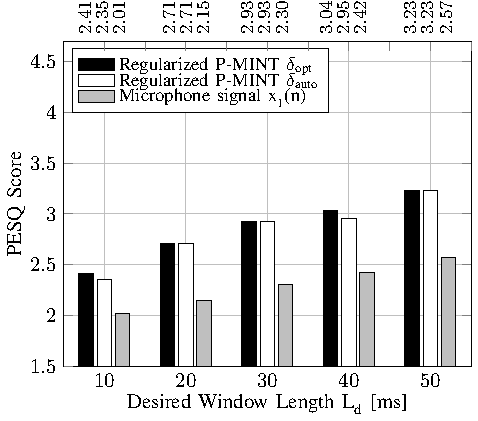
\includegraphics[scale=0.9]{figures/PESQ_optandautofixederror_sys_3_error_-15.pdf}
  \caption{PESQ score of the first microphone signal $x_1(n)$ and PESQ score of the system's output $\hat{s}(n)$ obtained for several $L_d$ using regularized P-MINT with $\delta_{\rm opt}$ and regularized P-MINT with $\delta_{\rm auto}$~($E_m = -15$~dB)}
  \label{fig: autopesq1}
\end{figure}
The PESQ scores obtained using the regularized P-MINT technique with the optimal and automatic regularization parameters for several desired window lengths and $E_m = -15$~dB are depicted in Fig.~\ref{fig: autopesq1}.
As illustrated in this figure, the performance when using $\delta_{\rm auto}$ is generally similar to the performance obtained when using $\delta_{\rm opt}$.
The average performance degradation over all considered $L_d$ is only $0.03$, implying that the automatic selection procedure for the regularization parameter provides a nearly optimal performance.
Furthermore, the normalized mean square error between the optimal and automatic regularization parameter over all considered $L_d$ is $0.03$, where the normalized error is defined as $(\log_{10}\delta_{\rm opt} - \log_{10}\delta_{\rm auto})/\log_{10}\delta_{\rm opt}$.

Since the optimal regularization parameter heavily depends on the channel mismatch and the considered acoustic system, we have also evaluated the performance when using $\delta_{\rm auto}$ for different $E_m$, i.e. $E_m \in \{ -33~{\rm dB}, \; -32~{\rm dB}, \; \ldots, \; -15~{\rm dB} \}$, and for different acoustic systems~($T_{\rm 60} \approx 450$~ms, $T_{\rm 60} \approx 550$~ms, $T_{\rm 60} \approx 750$~ms).
The desired window length in this simulation is set to $L_d = 50$~ms.
Fig.~\ref{fig: autopesq2} depicts the PESQ scores obtained using the optimal and the automatic selection procedure for the different normalized channel mismatch values and acoustic systems.
\begin{figure}[t!]
  \centering
  %\tikzsetnextfilename{auto_reg_Ld50_severalEm}
  %\input{Plots/auto_reg_Ld50_severalEm.tikz}
  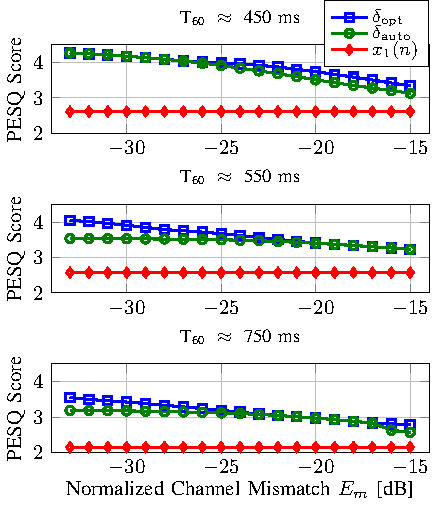
\includegraphics[scale=0.9]{figures/auto_reg_Ld50_severalEm.pdf}
  \caption{PESQ score of the first microphone signal $x_1(n)$ and PESQ score of the system's output $\hat{s}(n)$ obtained for different acoustic systems and several $E_m$ using regularized P-MINT with $\delta_{\rm opt}$ and regularized P-MINT with $\delta_{\rm auto}$~($L_d = 50$~ms)}
  \label{fig: autopesq2}
\end{figure}
It can be seen that for all considered acoustic systems and most channel mismatch values, very similar performance is achieved by both regularization parameters, whereas for some scenarios a small performance degradation can be noticed when using $\delta_{\rm auto}$.
The average performance degradation over all channel mismatch values when using $\delta_{\rm auto}$ is $0.11$~($T_{\rm 60} \approx 450$~ms), $0.18$~($T_{\rm 60} \approx 550$~ms), and $0.12$~($T_{\rm 60} \approx 750$~ms).
Furthermore, the normalized mean square error between the optimal and automatic regularization parameter over all channel mismatch values is $0.64$~($T_{\rm 60} \approx 450$~ms), $0.05$~($T_{\rm 60} \approx 550$~ms), and $0.05$~($T_{\rm 60} \approx 750$~ms).

Therefore, the presented results show that the automatic regularization parameter in P-MINT leads to a nearly optimal performance, making regularized P-MINT not only a robust and perceptually advantageous equalization technique, but practically applicable as well.

\subsection{Robustness in the Presence of Channel Estimation Errors and Additive Noise}
\label{sec: noise}
In this section we will investigate the performance of P-MINT and regularized P-MINT when using the non-intrusive regularization parameter $\delta_{\rm auto}$ in the presence of both channel estimation errors and additive noise $v_m(n)$, with $v_m(n)$ consisting of microphone self-noise and diffuse background noise recorded for the same acoustic scenario as in Section~\ref{sec: regacsys}.
More in particular, we will investigate the possible amplification of this additive noise when using reshaping filters that are designed without taking the presence of noise into account.

The noisy and reverberant signals $y_m(n)$ are generated by convolving the clean speech signal $s(n)$ with the true measured RIRs $h_m(n)$ and adding the recorded noise $v_m(n)$. 
The input broadband SNR averaged over all channels is ${\rm SNR}_{\rm av} = 15$~dB, with
\begin{equation}
  {\rm SNR}_{\rm av} = \frac{1}{M} \sum_{m = 1}^M 10 \log_{10} \left( \frac{\sum_{n} [x_m(n)]^2}{\sum_{n} [v_m(n)]^2}\right).
\end{equation}
Furthermore, the considered normalized channel mismatch between the true and estimated RIRs is $E_m = -15$~dB.
Hence, the same reshaping filters computed in the presence of only channel estimation errors using P-MINT and regularized P-MINT with $\delta_{\rm auto}$~(cf. Sections~\ref{sec: regacsys} and~\ref{sec: auto} respectively)  are applied to the received microphone signals $y_m(n)$.
\begin{table}[b!]
\centering
\caption{SNR improvement obtained for several $L_d$ using P-MINT and regularized P-MINT with $\delta_{\rm auto}$}
\label{tbl: snr}
\begin{tabular}{|l|r|r|r|r|r|r|r|}
\hline
$L_d$ [ms] & $10$ & $20$ & $30$ & $40$ & $50$ \\
\hline
P-MINT & $-11.24$ & $-23.11$ & $-25.20$ & $-31.22$ & $-19.59$  \\
\hline
Reg P-MINT & $-3.22$ & $4.39$ & $2.89$ & $0.39$ & $2.14$  \\
\hline
\end{tabular}

\end{table}
The performance at the output of the equalization system is evaluated in terms of the SNR improvement as well as in terms of the perceptual speech quality using PESQ.
Table~\ref{tbl: snr} presents the SNR improvement for different values of $L_d$ for both considered techniques.
The presented negative SNR improvement values show that P-MINT significantly amplifies the additive noise.
However, when regularization is incorporated, the robustness of regularized P-MINT to additive noise significantly increases, which can be explained by the fact that the energy of the reshaping filters is decreased.
When the energy of the reshaping filters is lower, the amplification of the undesired noise term in the output signal is also smaller~(cf.~(\ref{eq: 3})).
Furthermore, Table~\ref{tbl: pesq} depicts the obtained PESQ scores, where it can be seen that P-MINT leads to a lower perceptual speech quality than the received microphone signal $y_1(n)$. 
However, the automatically regularized P-MINT technique yields a higher perceptual speech quality, with a significant improvement over $y_1(n)$.
\begin{table}[t!]
\centering
\caption{PESQ score of the first microphone signal $y_1(n)$ and PESQ score of the system's output $\hat{s}(n)$ obtained for several $L_d$ using P-MINT and regularized P-MINT with $\delta_{\rm auto}$}
\label{tbl: pesq}
\begin{tabular}{|l|r|r|r|r|r|r|r|}
\hline
$L_d$ [ms] & $10$ & $20$ & $30$ & $40$ & $50$ \\
\hline
P-MINT & $1.65$ & $1.83$ & $1.78$ & $2.03$ & $2.29$  \\
\hline
Reg P-MINT & $2.25$ & $2.60$ & $2.79$ & $2.81$ & $3.07$  \\
\hline
$y_1(n)$ & $1.99$ & $2.11$ & $2.27$ & $2.39$ & $2.52$  \\
\hline
\end{tabular}

\end{table}

These simulation results show that regularization is effective in P-MINT not only to increase robustness to channel estimation errors, but also to avoid amplification of the additive noise present at the microphones. 
\section{Conclusion}
In this paper we introduced the partial multichannel equalization technique P-MINT, which aims to suppress the reverberant tail of the RIR as well as to directly control the perceptual speech quality.
Furthermore, we presented a robust extension to P-MINT and other recently proposed multichannel equalization techniques, i.e. RMCLS and CS, by incorporating a regularization term in the reshaping filter design.
In addition, we proposed an automatic non-intrusive selection procedure for the regularization parameter which leads to a nearly optimal perceptual speech quality.

We have extensively investigated the effectiveness of regularization both in terms of reverberant tail suppression and perceptual speech quality for all considered equalization techniques.
Simulation results show that the regularized P-MINT technique with the intrusively determined regularization parameter leads to the highest robustness and perceptual speech quality.
Furthermore, simulation results demonstrate that regularization is particularly important for P-MINT, whereas for RMCLS and CS a smaller performance improvement is achieved.
Finally, it is shown that the automatic non-intrusive procedure for the selection of the regularization parameter yields a nearly optimal perceptual speech quality in regularized P-MINT.


\bibliographystyle{IEEEtran}
\bibliography{refs}



\begin{IEEEbiography}[{
\includegraphics[width=1in,height=1.25in,clip,keepaspectratio]{figures/Ina_Kodrasi}}]
{Ina Kodrasi}~(S'11) received the Master of Science degree in Communications, Systems and Electronics in 2010 from Jacobs University Bremen, Bremen, Germany.
Since 2010 she is a PhD student at the Signal Processing Group of the University of Oldenburg, Germany.
Her research interests are in the area of signal processing for speech and audio applications.

From 2010 to 2011 she was with the Fraunhofer Institute for Digital Media Technology (IDMT), Project group
Hearing, Speech and Audio Technology in Oldenburg where she worked on microphone-array beamforming.
\end{IEEEbiography}

\begin{IEEEbiography}[{
\includegraphics[width=1in,height=1.25in,clip,keepaspectratio]{figures/Stefan_Goetze}}]
{Stefan Goetze} is head of Audio System Technology for Assistive Systems at the Fraunhofer Institute for Digital Media Technology (IDMT), Project group Hearing, Speech and Audio (HSA) in Oldenburg, Germany.
He received his Dipl.-Ing. in 2004 at the University of Bremen, Germany, where he worked as a research engineer from 2004 to 2008.
His research interests are assistive technologies, sound pick/up and enhancement, such as noise reduction, acoustic echo cancellation and dereverberation, as well as detection and classification of acoustic events and automatic speech recognition.
He is lecturer at the University of Bremen and project leader of national and international projects in the field of ambient assisted living (AAL).
He is member of IEEE and AES.
\end{IEEEbiography}

\begin{IEEEbiography}[{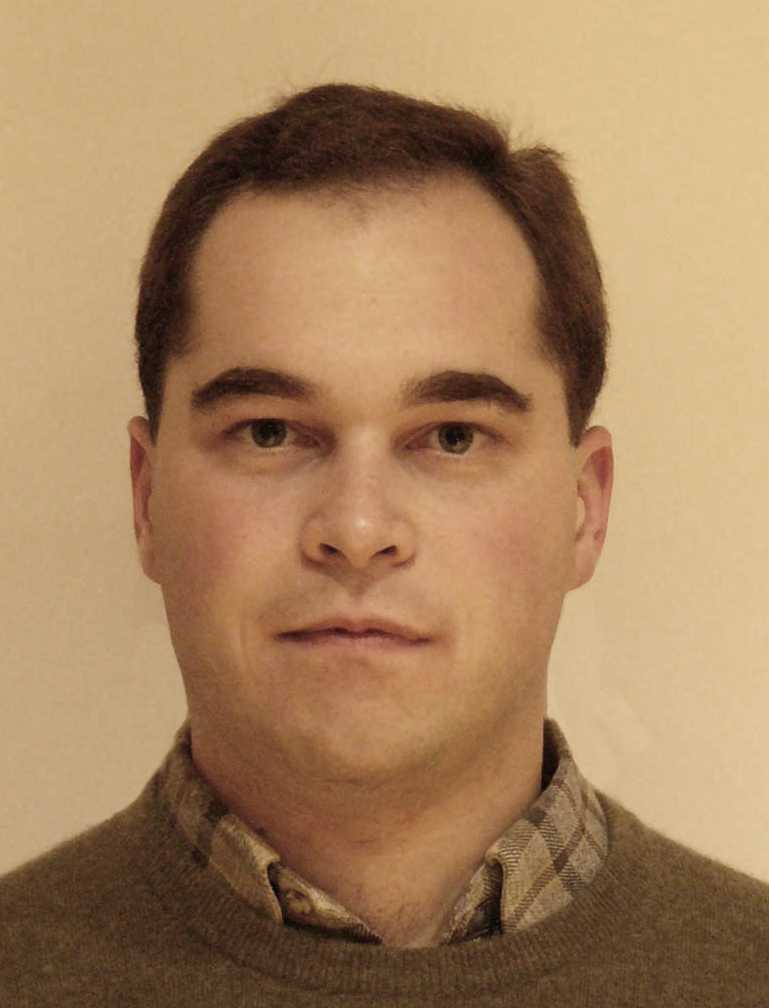
\includegraphics[width=1in,height=1.25in,clip,keepaspectratio]{figures/Simon_Doclo}}]{Simon Doclo}
(S'95, M'03) received the M.Sc. degree in electrical engineering and the Ph.D. degree in applied sciences from the Katholieke Universiteit Leuven, Belgium, in 1997 and 2003. From 2003 to 2007 he was a Postdoctoral Fellow with the Research Foundation – Flanders at the Electrical Engineering Department (Katholieke Universiteit Leuven) and the Adaptive Systems Laboratory (McMaster University, Canada). From 2007 to 2009 he was a Principal Scientist with NXP Semiconductors at the Sound and Acoustics Group in Leuven, Belgium. Since 2009 he is a full professor at the University of Oldenburg, Germany, and scientific advisor for the project group Hearing, Speech and Audio Technology of the Fraunhofer Institute for Digital Media Technology. His research activities center around signal processing for acoustical applications, more specifically microphone array processing, active noise control, acoustic sensor networks and hearing aid processing.
Prof. Doclo received the Master Thesis Award of the Royal Flemish Society of Engineers in 1997 (with Erik De Clippel), the Best Student Paper Award at the International Workshop on Acoustic Echo and Noise Control in 2001, the EURASIP Signal Processing Best Paper Award in 2003 (with Marc Moonen) and the IEEE Signal Processing Society 2008 Best Paper Award (with Jingdong Chen, Jacob Benesty, Arden Huang). He is a member of the IEEE Signal Processing Society Technical Committee on Audio and Acoustic Signal Processing (2008-2013). He has been secretary of the IEEE Benelux Signal Processing Chapter (1998-2002), and has served as a guest editor for the EURASIP Journal on Applied Signal Processing.
\end{IEEEbiography}

\end{document}

